\section{One-loop neutrino masses}
\label{sec:mass-interaction-basis}

By using the Feynman rules for Weyl spinors we have the diagrams for
neutrino masses at 1-loop shown in \ref{fig:t13aweyl}
\begin{figure}
  \centering
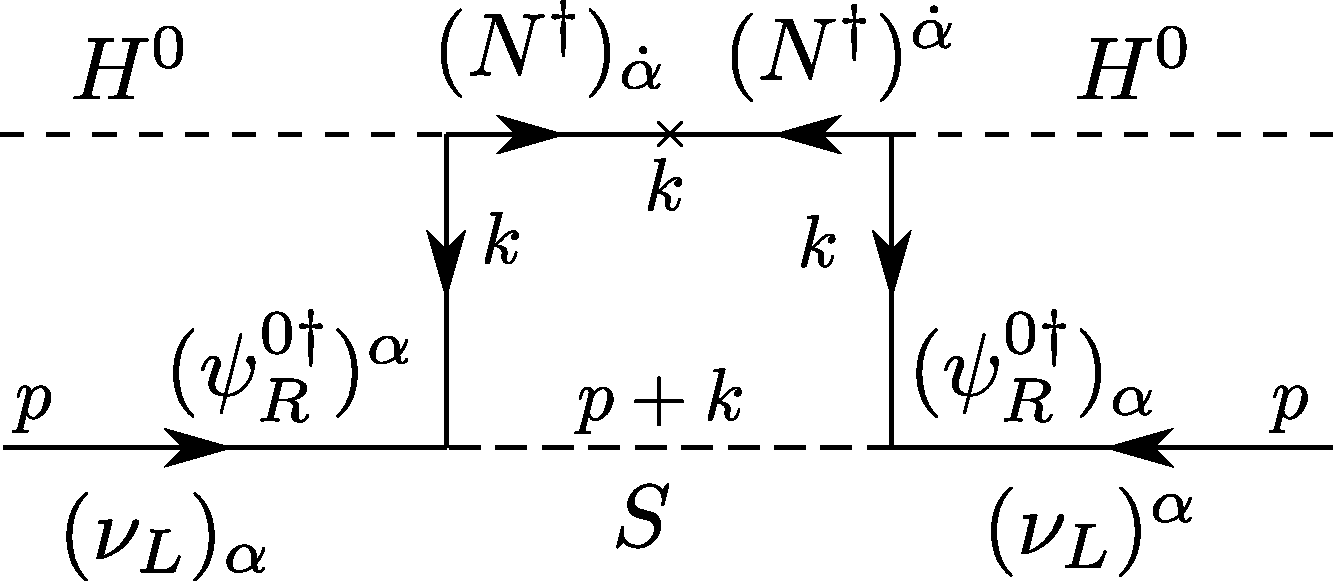
\includegraphics[scale=0.3]{T13AweylR}\qquad 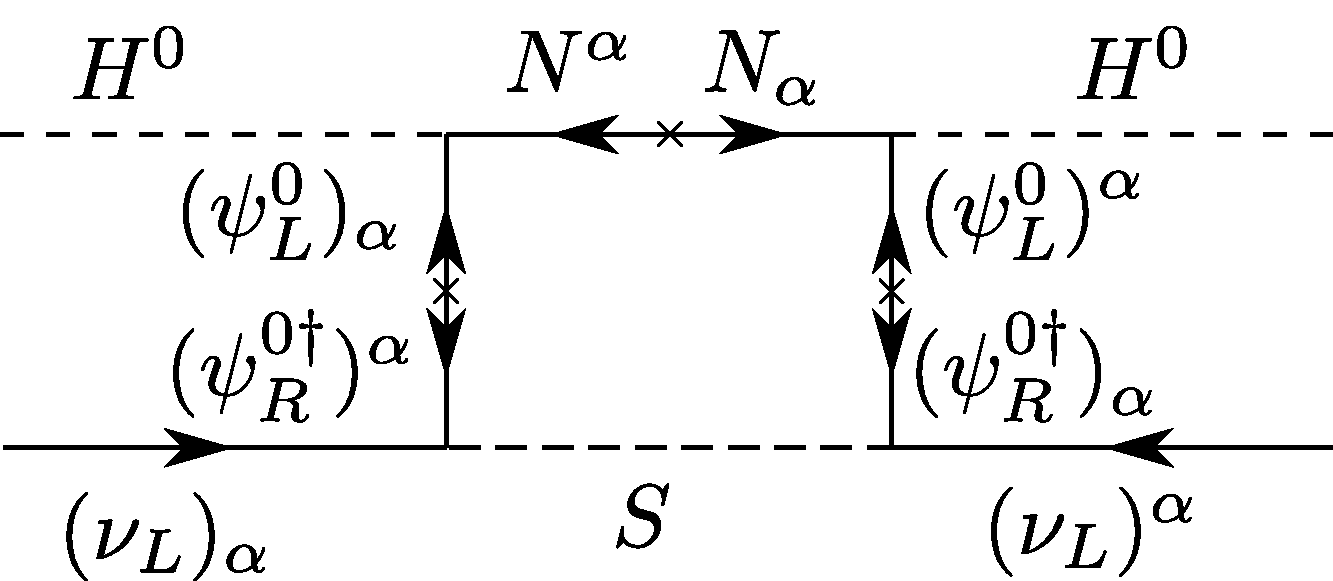
\includegraphics[scale=0.3]{T13AweylRL}
  \caption{1-loop neutrino mass in the interaction basis}
  \label{fig:t13aweyl}
\end{figure}

The results from \cite{Bonnet:2012kz,Suematsu:2010nd} adapted to our case imply that ($\lambda_d \to Y_L\; \lambda_u \to Y_R$)
%check nuint.pdf
\begin{align}
  M^{\nu}_{ij}=2\sum_{\alpha}h_{i\alpha}h_{j\alpha} &\left[  \lambda_u^2\int \frac{d^4 k}{(2\pi)^4}i S_F \left(k,M_D \right)P_R S_F \left(k,M_N \right)P_R i S_F \left(k,M_D \right)
             \Delta_F \left( k+p,m_{S_\alpha} \right)\right. \nonumber\\
          &\left.+\lambda_d^2\int \frac{d^4 k}{(2\pi)^4}i S_F \left(k,M_D \right)P_L S_F \left(k,M_N \right)P_L i S_F \left(k,M_D \right)
             \Delta_F \left( k+p,m_{S_\alpha} \right) 
            \right].
\end{align}

\begin{align}
  M^{\nu}_{ij}=\sum_{\alpha}\frac{2h_{i\alpha}h_{j\alpha}v^2 M_N}{(4\pi)^2} 
      \left[\lambda_u^{2} \, J_4\left(M_D^2,M_D^2,M_N^2,m^{S}_{\alpha}  \right)
            + \lambda_d^2 M_D^2  \, I_4\left(M_D^2,M_D^2,M_N^2,m^2_{S_\alpha}  \right)
      \right],
\end{align}
where
\begin{align}
   J_4\left(M_D^2,M_D^2,M_N^2,m^2_{S}  \right)=&\frac{(4\pi)^2}{i}
   \int \frac{d^4 k}{(2\pi)^4}
\frac{k^2}{\left(k^2-m_D^2\right)^2\left( k^2-M_N^2 \right)\left(k^2-m_{S_\alpha}^2\right)} \nonumber\\
   I_4\left(M_D^2,M_D^2,M_N^2,m^2_{S}  \right)=&\frac{(4\pi)^2}{i}
   \int \frac{d^4 k}{(2\pi)^4}
\frac{1}{\left(k^2-m_D^2\right)^2\left( k^2-M_N^2 \right)\left(k^2-m_{S_\alpha}^2\right)}.
\end{align}
After integration
%see calculoij.pdf
\begin{align*}
  J_4\left(M_D^2,M_D^2,M_N^2,m^2_{S}  \right)=
-&\left\{  \left[\frac{M_D^2}{\left(M_N^2-M_D^2\right)\left(m_{S}^2-M_D^2\right)} 
-\frac{M_D^4 \left(2M_D^2-M_N^2-m_{S_\alpha}^2\right)}{2\left(M_N^2-M_D^2\right)^2\left(m_{S}^2-M_D^2\right)^2} \right]\ln M_D^2\right.\nonumber\\
&-\frac{M_N^4\ln M_N^2}{2\left( m_{S_\alpha}^2-M_N^2 \right)\left( M_D^2-M_N^2 \right)^2}-
\frac{m_{S_\alpha}^4\ln m_{S_\alpha}^2}{2\left( m_N^2-m_{S_\alpha}^2 \right)\left( M_D^2-m_{S_\alpha}^2 \right)^2}
\nonumber\\
 &\left.+\frac{M_D^2}{2\left(M_N^2-M_D^2  \right)\left(m_{S_\alpha}^2-M_D^2  \right)} \right\},
\end{align*}
\begin{align}
      I_4&\left(M_D^2,M_D^2,M_N^2,m^2_{S}  \right)=\nonumber\\
&\left[\frac{M_N^2\ln \left( M_N^2/M_D^2 \right)}{\left( M_N^2-M_D^2 \right)^4\left( M_N^2-m_{S_\alpha}^2 \right)^2}
      -\frac{m_{S_\alpha}^2\ln \left( m_{S_\alpha}^2/M_D^2 \right)}{\left( m_{S_\alpha}^2-M_D^2 \right)^4\left( M_N^2-m_{S_\alpha}^2 \right)^2}-
      \frac{1}{\left(m_{S_\alpha}^2-M_D^2\right)^2\left(M_N^2 -M_D^2 \right)^2} 
 \right],
\end{align}
or
\begin{align}
   I_4\left(M_D^2,M_D^2,M_N^2,m^2_{S}  \right)=
-&\left[ \frac{\left(M_D^4-M_N^2 m_{S_\alpha}^2\right)\ln M_D^2}{\left(M_N^2 -M_D^2 \right)^2\left(m_{S_\alpha}^2 -M_D^2 \right)^2} 
+\frac{M_N^2 \ln M_N^2}{\left(m_{S_\alpha}^2 -M_N^2 \right)\left(M_D^2-M_N^2\right)^2}\right. \nonumber\\
&\left.+\frac{m_{S_\alpha}^2 \ln m_{S_\alpha}^2}{\left(M_N^2 -m_{S_\alpha}^2 \right)\left(M_D^2-m_{S_\alpha}^2\right)^2} 
-\frac{1}{\left(m_{S_\alpha}^2-M_D^2\right)\left(M_N^2 -M_D^2 \right)} 
\right].
\end{align}

In  \cite{Fraser:2014yha} only the contribution proportional to $\lambda_u$ is considered in the limit $M_N\to 0$\footnote{$\lim_{x\to 0}x\ln x=\lim_{x\to 0}\dfrac{\ln x}{1/x}=0$}, 
\begin{align*}
   J_4\left(M_D^2,M_D^2,M_N^2,m^2_{S}  \right)=&
-\left\{  \left[-\frac{M_D^2}{M_D^2\left(m_{S}^2-M_D^2\right)} 
-\frac{M_D^4 \left(2M_D^2-m_{S_\alpha}^2\right)}{2M_D^4\left(m_{S}^2-M_D^2\right)^2} \right]\ln M_D^2\right.\nonumber\\
&\qquad+\frac{m_{S_\alpha}^4\ln m_{S_\alpha}^2}{2m_{S_\alpha}^2\left( M_D^2-m_{S_\alpha}^2 \right)^2} 
\left.-\frac{M_D^2}{2M_D^2\left(m_{S_\alpha}^2-M_D^2  \right)} \right\}\nonumber\\
=&  -\left\{  -\left[\frac{1}{\left(m_{S}^2-M_D^2\right)} 
+\frac{\left(2M_D^2-m_{S_\alpha}^2\right)}{2\left(m_{S}^2-M_D^2\right)^2} \right]\ln M_D^2
+\frac{m_{S_\alpha}^2\ln m_{S_\alpha}^2}{2\left( M_D^2-m_{S_\alpha}^2 \right)^2} 
-\frac{1}{2\left(m_{S_\alpha}^2-M_D^2  \right)} \right\}\nonumber\\
=&  -\frac{1}{\left(m_{S}^2-M_D^2\right)}\left\{  -\left[1 
+\frac{\left(2M_D^2-m_{S_\alpha}^2\right)}{2\left(m_{S}^2-M_D^2\right)} \right]\ln M_D^2
+\frac{m_{S_\alpha}^2\ln m_{S_\alpha}^2}{2\left( M_D^2-m_{S_\alpha}^2 \right)} 
-\frac{1}{2} \right\}\nonumber\\
= & \frac{1}{2\left(m_{S}^2-M_D^2\right)}\left\{  \frac{m_{S_\alpha}^2\ln M_D^2}{\left(m_{S}^2-M_D^2\right)}
-\frac{m_{S_\alpha}^2\ln m_{S_\alpha}^2}{\left( M_D^2-m_{S_\alpha}^2 \right)} +1 \right\}\nonumber\\
=&  \frac{1}{2\left(m_{S}^2-M_D^2\right)}\left[ 1+ \frac{m_{S_\alpha}^2\ln \left( M_D^2/m_{S_\alpha}^2 \right)}{\left(m_{S}^2-M_D^2\right)}
\right]\nonumber\\
=& - \frac{1}{2\left(M_D^2-m_{S}^2\right)}\left[ 1-\frac{m_{S_\alpha}^2\ln \left( M_D^2/m_{S_\alpha}^2 \right)}{\left(M_D^2-m_{S}^2\right)}
\right].
\end{align*}
So that
\begin{align*}
M^{\nu}_{ij}=-\sum_{\alpha}\frac{h_{i\alpha}h_{j\alpha}\left(\lambda_u^2 v^2\right)M_N}{16\pi^2\left(M_D^2-m_{S_\alpha}^2\right)}
\left[ 1-\frac{m_{S_\alpha}^2\ln \left( M_D^2/m_{S_\alpha}^2 \right)}{\left(M_D^2-m_{S_\alpha}^2\right)}\right].
\end{align*}